\sectioncentered*{Аннотация}
\thispagestyle{empty}

\begin{center}
  \begin{minipage}{0.82\textwidth}
    на дипломный проект <<Android-приложение: агрегатор игровых магазинов>> студента УО <<Белорусский государственный университет информатики и радиоэлектроники>> Демидовича~И.\,В.
  \end{minipage}
\end{center}

\emph{Ключевые слова}: приложение, мобильное, магазин, игры, предложение.
\vspace{1\parsep}

Целью дипломного проекта является разработка мобильного приложения, которое должно облегчить процесс поиска лучших предложений среди игровых магазинов на рынке.

Первый раздел содержит обзор предметной области, разбор аналогов создаваемого программного продукта. На основе проведенного анализа формулируются требования к проектируемому программному продукту.

В втором разделе производится обзор технологий, использованных для реализации программного продукта.

В третьем разделе проводится моделирование предметной области и разработка требований для программного продукта.

Четвертый раздел посвящен проектированию архитектуры приложения. В нём рассмотрены основные модули и компоненты, которые необходимо реализовать в программном продукте.

В пятом разделе дано описание процесса разработки программного продукта в рамках дипломного проекта, описания основных особенностей реализации, примеры использования и информация о тестировании.

В шестом разделе предоставлено технико-экономическое обоснование эффективности разработки программного продукта.

В заключении подводятся итоги проделанной работы и делаются выводы по дипломному проекту. Также описывается дальнейший план развития проекта.

Дипломный проект выполнен самостоятельно и проверен в системе «Антиплагиат». Цитирования обозначены ссылками на публикации, указанные в «Списке литературы».
\begin{figure}[H]
  \centering
    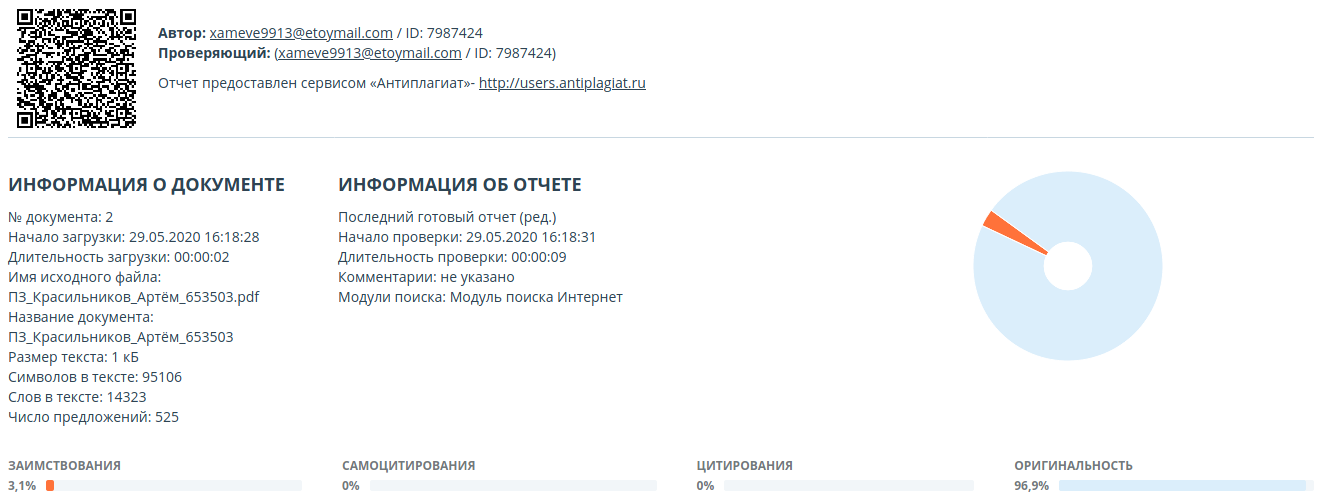
\includegraphics[scale=0.3]{anti.png} 
    \label{fig:anti}
 \end{figure}
\clearpage